

\section{ELMo (Embeddings from Language Models)}


\begin{frame}{ELMo: Motivation}
    \large \linespread{0.4}
    
    \textbf{Motivation for ELMo: }Remember \textbf{polysemy}? Contextual embeddings create one vector per word type in a context. 
    
    \begin{exampleBlock}{Example}
        If instead models used only word and character embedding, the homonyms ``book" (text) and ``book" (reservation) are assigned the \emph{same vector representation even though these are different words}. 
        
        This vector representation may of course be created using context (as from Word2Vec or GloVe) but contextual meanings get \emph{collapsed into a single representation}.
    \end{exampleBlock}
    
    
\end{frame}



\begin{frame}{ELMo: Structure}

    \begin{itemizeSpaced}{2pt}
        \pinkbox \textbf{ELMo} uses bidirectional language model (biLM) to make \emph{deep} word embeddings (derived from all its internal layers)

        \pinkbox Higher-level LSTM layers capture contextual meaning (useful for supervised word sense disambiguation (WSD)).
        
        \pinkbox Lower layers capture syntax information (useful for part of speech tagging (POS)). 
        
        \pinkbox Mixing these signals let ELMo's embeddings select the types of semi-supervision most needed for each end task $\Rightarrow$ ELMo embeddings are thus richer than traditional word vectors. 
        
        \item \textbf{Task-Specific: } ELMo is a task-specific combination of the intermediate layer representations in the biLM (collapses forward and backward hidden states into single embedding for a specific task by weighting the biLM layers): \footnotemark 
        $$
        \textbf{ELMo}_k^{task} = E \Big( R_k; \theta^{task} \Big) = \gamma^{task} \; \sum_{j=0}^L s_j^{task} \; \mathbf{h}_{kj}^{LM}
        $$ 
        
        
    \end{itemizeSpaced}
    
    \footnotetext[10]{ \footnotesize the vector $\mathbf{s}^{task} = \Big\{ s_j^{task} \Big\}$ of softmax-normalized weights and task-dependent scalar parameter $\gamma^{task}$ allow the model for the specific $task$ to scale the entire $\textbf{ELMo}_k^{task}$ vector. The index $k$ corresponds to a $k$-th word, and index $j$ corresponds to the $j$-th layer out of $L$ layers. Here, $h_{kj}^{LM}$ is the output of the $j$-th LSTM for word $k$, and $s_j$ is the weight of $h_{kj}^{LM}$ used to compute the representation for word $k$. }
    
    
\end{frame}



\begin{frame}{ELMo: Example and Key Feature}
    
    
    
    \begin{table}[ht!]
      \centering
      \begin{tabular}{ c }
        
        \begin{minipage}{.9\textwidth}
          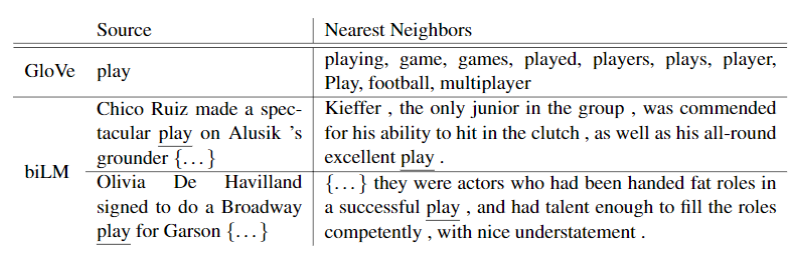
\includegraphics[width=\linewidth]{imgs/table_elmoPlay.png}
        \end{minipage}
        \vspace{-7pt}
      \end{tabular}
      \caption{\linespread{0.3} \scriptsize Nearest neighbors to ``play” using GloVe and the context embeddings from a biLM. From \emph{Table 4 in Deep Contextualized Word Representations}, by Peters et al., 2018. \url{https://arxiv.org/pdf/1802.05365.pdf}. Copyright 2018 by Peters et al.}
      \label{tbl:elmoPlayExample}
      \vspace{-10pt}
    \end{table}
    
    
    {\linespread{0.3}
    \begin{itemizeSpaced}{4pt}
        
        \item \cref{tbl:elmoPlayExample} displays words nearest to polysemous word ``play" found using GloVe vs biLM. 
        
        \pinkbox GloVe's neighbors have different parts of speech, like verbs (``played", ``playing"), and nouns (``player", ``game") and only in the sport sense.
        
        
        \pinkbox biLM's nearest neighbor sentences from ``play'' CWE show clear difference between \emph{both} the parts of speech \emph{and} word sense of ``play". 
        
        \begin{itemizeSpaced}{0pt}
            \pinkbox last row: input sentence has noun / acting sense of ``play" and this is matched in the nearest neighbor sentence
        \end{itemizeSpaced}        
            
    
    \end{itemizeSpaced} }
    
    \textbf{ELMo key feature: } learn context using part of speech tagging (POS) and word sense disambiguation (WSD).  
    
\end{frame}